% Chapter Template

\chapter{Morphing of Local Statistics: Mapping Through a Resolution Bottleneck} % Main chapter title
\label{Morphing:intro}

Top-down coarse-grained (CG) models are designed to study the implications of general rules, which are typically inferred from universal physical principles or constructed to reproduce specific phenomena. Unlike bottom-up CG models, top-down models are not build upon a higher resolution model. However, top-down models can still be related to a specific chemistry. To this end, the deployed interaction potentials are tuned in order to reproduce certain properties of a target system, such as density \cite{shelley2001simulations}, interfacial tension \cite{shinoda2007multi} or partitioning of compounds between aqueous and hydrophobic environments \cite{marrink2004coarse}.  

An example of such chemically-specific top-down models is the Kremer-Grest (KG) polymer model with an additional bending potential \cite{kremer1990dynamics, grest1986molecular, faller1999local}. A relation to real polymers can be established by matching the experimentally observed Kuhn number, which is a key parameter to characterize a specific polymer chemistry \cite{everaers2020kremer, svaneborg2020characteristic}. Such Kuhn scale matched model polymers can be regarded as a special case of structure-based coarse-graining: Controlling the Kuhn number with the parameter for the chain stiffness allows for a reproduction of emergent universal large length- and time-scale behavior. However, while this remarkable simple model is able to retain the behavior above the Kuhn scale, particular properties below the Kuhn scale, i.e. local properties, are not expected to resemble the target system \cite{everaers2020kremer}. Specifically, solely structure-based CG models on a similar level of resolution are presumed to yield a locally more faithful representation.

In this chapter, a machine learning (ML) method to adjust local properties of molecular structures is introduced. In particular, two distributions of molecular configurations are considered, 1) a distribution of configurations sampled from a top-down CG model, which will be referred to as top-down distribution in the following, and 2) a target distributions, which denotes more faithful representations of the same molecular system. It is assumed that molecular configurations from both distributions share large-scale properties, but differ locally. To improve the quality of the top-down distribution, a ML model is trained to transform it, such that it resembles the target distribution more closely. To this end, the ML model is trained to reproduce local correlations learned from the target distribution, while large-scale properties are maintained. This adjustment of local features based on a target distribution will be referred to as \textit{morphing} in the following.

%The approach is illustrated in Fig.~\ref{FIG:morph_intro}. Morphing is performed by deepbackmap (DBM), which is outlined in Chpt. \ref{methology}. To this end, a local scale is introduced that defines the extent to which features are morphed. Specifically, molecular structures are further CG up to this scale. DBM is trained on the target distribution to reintroduce details for such CG structures. Afterwards, the trained model is transferred to the distribution of the top-down model to reproduce local properties learned from the target distribution.

The motivation for this project is to introduce a two-step backmapping scheme for top-down CG models. A mismatch of local properties on the CG scale between the top-down distribution and a particular target system can impact the quality of backmapped structures, i.e. unphysical artifacts at the higher resolution are expected to occur more frequently. In order to reduce such artifacts already on the CG scale, local statistics of the CG structure are corrected before serving it as an input for the backmapping algorithm. 

In the following, the method is applied to two systems: (1) A polymer melt of syndiotactic polystyrene (sPS) sampled with the KG model with tuned bending potential and (2) a condensed-phase system of the alkane tetracosane (TCS) sampled with the Martini force field \cite{marrink2007martini}. The content presented in this chapter is not published yet.

\label{morphing} % Change X to a consecutive number; for referencing this chapter elsewhere, use \ref{ChapterX}

\section{Method}
\label{Morphing:method}

\begin{figure}
  \centering
      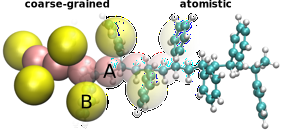
\includegraphics[width=1.0\textwidth]{./Figures/morphing/intro.pdf}
  \caption{Illustration of the morphing approach: Molecular structures from a distribution $\mathcal{X}$ are mapped through a resolution bottleneck in order to reinsert local features learned from a target distribution $\mathcal{Y}$. To this end, a local scale $s$ is introduced defining the extent to which features are varied. In particular, an encoder $e_s$ is applied to map molecular configurations to a lower resolution and a backmapping model $g_s$ is utilized to reinsert details. Importantly, training of $g_s$ is fixed to the target distribution $\mathcal{Y}$. Afterwards, the trained model is transferred to $\mathcal{X}$. Choosing the value for $s$ is a trade-off between the complexity of the backmapping task and the impact of the morphing.}
  \label{FIG:morph_intro}
\end{figure}

The method applied in this chapter aims at morphing local features of molecular structures by passing them through a resolution bottleneck. The idea is inspired by the concept of cross-modal learning (CML) known in the ML community \cite{feng2014cross, cao2016correlation, mukherjee2017deep, yoo2019image}. CML is used to link sources of information from different domains, such as audio-to-image translation. As an instructive example, consider two distributions $\mathcal{A}$ and $\mathcal{B}$ that refer to audio signals and images, respectively. In order to map an audio signal to the domain of images, two autoencoders $A$ and $B$ are trained to encode and decode elements $\mathbf{a}$ and $\mathbf{b}$ sampled from $\mathcal{A}$ and $\mathcal{B}$, respectively. In its core, a link between both distributions can be established by matching the encoded distributions in the latent space. In particular, mapping between $\mathcal{A}$ and $\mathcal{B}$ is performed by cross-connecting the encoder $e$ and decoder $d$ of both models, i.e. $d_B\big(e_A(\mathbf{a})\big)$ for audio-to-image translation. However, connecting the latent distributions of both models, i.e. the information-bottleneck, is challenging and subject to current research \cite{wang2016comprehensive}.

Here, two distributions of molecular structures $\mathcal{X}$ and $\mathcal{Y}$ are given that both represent the same molecular system at an equivalent resolution. It is assumed that molecular configurations of both distributions display similar large-scale features, but differ in their local properties. In the following, $\mathcal{X}$ denotes the distribution of a top-down CG model, while $\mathcal{Y}$ denotes a target distribution representing more faithful molecular structures, for example obtained by a structure-based CG method. In order to map from $\mathcal{X}$ to $\mathcal{Y}$, a ML-based function $g$ is introduced to learn the transformation $g(\mathcal{X}) \approx \mathcal{Y}$. As displayed in Fig.~\ref{FIG:morph_intro}, a similar idea to CML is applied and both distributions are matched at a lower-resolution, i.e. at an information-bottleneck. To this end, a simple encoder $e_s$ is chosen that reduces the number of particles $n$ by a factor $s$

%However, both distributions differ, for example because of a mismatch of their underlying force fields.
\begin{equation}
 e_{s}: \mathbb{R}^{3n} \rightarrow \mathbb{R}^{3n/s} ,
\end{equation}

, i.e. $e_s$ denotes a fine-to-coarse mapping of the coordinates. Specifically, $e_s$ computes the center of mass for groups of $s$ particles. Afterwards, encoded structures are backmapped to the original resolution deploying the ML model $g_s$, such that $g_s(e_s \big( \mathcal{Y} \big) ) = \mathcal{Y}$. To this end, $g_s$ is trained with the deepbackmap (DBM) approach, which is introduced in Chpt. \ref{methology}. Importantly, training of $g_s$ is fixed to the target distribution $\mathcal{Y}$. Afterwards, the trained model is transferred to $\mathcal{X}$ to perform the morphing $g_s(e_s \big( \mathcal{X} \big) ) \approx \mathcal{Y}$, i.e. to reinsert local correlations into the CG structures $e_s(\mathcal{X})$ learned from $\mathcal{Y}$.

%. As such, local correlations learned from $\mathcal{Y}$ are reinserted into the CG structures $e(\mathcal{X})$

%While the ultimate goal is to introduce a ML based mapping function $g_{\Theta}$ from one distribution to the other, i.e. $g_{\Theta}(\mathcal{X}) \approx \mathcal{Y}$, it is investigated if such a mapping can be realized by changing features only on a local scale. In other words, it is hypothesized that both distributions match at a lower resolution. To this end, a simple encoder $e_s$, i.e. a fine-to-coarse mapping of the coordinates, is chosen that reduces the number of particles $n$ by a factor $s$

%\begin{equation}
% e_{s}: \mathbb{R}^{3n} \rightarrow \mathbb{R}^{3n/s} .
%\end{equation}

%Specifically, $e_n$ computes the center of mass for groups of $n$ particles. Afterwards, the CG structure is backmapped utilizing DBM as explained in Sec. \ref{methology}. Similarly to the idea of CML, DBM is trained solely on structures drawn from the target distribution $\mathcal{Y}$ but deployed for CG structures drawn from the model distribution $\mathcal{X}$. As such, local features removed by $e_s$ are reinserted based on the local correlations learned from $\mathcal{Y}$. 

The value for the coarse-graining factor $s$ scales the extent to which local features are varied. Assuming that the backmapping scheme yields a perfect reconstruction, the mapping $g_s(e_s(\mathcal{X}))$ is expected to yield a more accurate reproduction of $\mathcal{Y}$ the larger $s$ becomes, since the reinsertion of details becomes less restricted by the CG representation $e_s(\mathcal{X})$. However, larger values of $s$ lead to a more complex backmapping exercise. As such, choosing the value for $s$ is a trade-off between the complexity of the backmapping task and the impact of the morphing. 

Two different morphing schemes A and B, respectively, are tested in this work. Scheme A refers to the basic backmapping protocol outlined in Chpt. \ref{methology}, i.e. the method deploys forward sampling to obtain an initial high-resolution structure, which is further refined applying Gibbs sampling. In contrast, scheme B skips the forward sampling step and utilizes the original high-resolution structure drawn from $\mathcal{X}$ as an initial structure, i.e. only Gibbs sampling is applied.

The proposed method is data driven, as the morphing is learned from training data, and does not require to parameterize a force field for the given target distribution. However, the quality of morphed structures can be improved by incorporating a simple potential energy during training of the ML model that penalizes certain configurations in terms of bond lengths, angles and non-bonded distances. An illustration of such a potential energy landscape can be found in Fig. \ref{FIG:morph_energy}. In particular, a harmonic potential of the form

\begin{figure}
  \centering
      \includegraphics[width=0.5\textwidth]{./Figures/morphing/energy.pdf}
  \caption{ Illustration of a simple energy landscape for bonded interactions to improve the quality of morphed molecular structures. $\phi$ represents bond lengths or angles, $\phi_{\text{min}}$ and $\phi_{\text{max}}$ are the minimum and maximum values obtained from the distribution $p(\phi)$, and $U(\phi)$ is a harmonic potential to penalize regions below $\phi_{\text{min}}$ or above $\phi_{\text{max}}$.}
  \label{FIG:morph_energy}
\end{figure}

\begin{equation}
 U(\phi) =
  \begin{cases}
      a(\phi - \phi_{\text{min}})^2,& \phi < \phi_{\text{min}}\\
      a(\phi - \phi_{\text{max}})^2,& \phi > \phi_{\text{max}}\\
      0,              & \text{otherwise},
  \end{cases}
\end{equation}

is applied as bonded interaction, where $\phi$ represents bond lengths or angles, respectively, $a$ is a scaling factor, and $\phi_{\text{min}}$/$\phi_{\text{max}}$ are threshold values of the potential. Similarly, a harmonic potential for non-bonded distances $d$

\begin{equation}
 U(d) =
  \begin{cases}
      a(1 - \frac{d}{d_{\text{min}}})^2,& d < d_{\text{min}}\\
      0,              & \text{otherwise},
  \end{cases}
\end{equation}

is introduced, where $d_{\text{min}}$ is the minimum distance for non-bonded particles. The values for the minimum and maximum distances/angles are obtained from the target distribution.

\section{Set-up and Reference Data}

The morphing approach is applied to a sPS polymer melt sampled with the KG model with tuned bending potential and a condensed-phase system of the alkane tetracosane sampled with the Martini force field. In addition, a higher resolution model is deployed for each system in order to obtain locally more faithful molecular structures that serve as a target distribution, which is used to train the ML model.

\subsection{Kremer-Grest Model: Syndiotactic Polystyrene}
\label{Morphing:KG}

The KG model is a standard model for computer simulations of polymeric systems \cite{kremer1990dynamics, grest1986molecular}. It is designed to study generic polymer properties with an emphasize on computational efficiency and simplicity. As outlined in Sec. \ref{Theory_MS:cg_methods}, the KG model is a bead-spring model, where consecutive beads are connected via strong nonlinear springs, i.e. the FENE potential (Eq. \ref{KG_fene}), and mutual interactions between all beads are modeled via a truncated Lennard-Jones potential (Eq. \ref{KG_wca}). The deployed interaction potentials are tuned such that topological constraints found in real polymeric systems are reproduced, i.e. chain backbones are prohibited to pass through each other. As such, the KG model is able to yield large scale entanglement properties that are characteristic for long-chain polymers. In order to modify the stiffness of the polymer chains, an additional bending potential can be introduced (Eq. \ref{KG_bending}), which is scaled by a prefactor $\kappa$ \cite{faller1999local}.

\subsubsection{Matching at the Kuhn Scale}

An important characteristic of many polymeric systems is their universal large-scale behavior that manifests in scaling relations. Specifically, the \textit{mean square end-to-end distance} $\langle R^2_e \rangle$ of a polymer chain scales with the number of beads $N$, i.e. $\langle R^2_e \rangle \propto N^{2\nu}$. In a melt state, polymers adopt the characteristics of a random-walk and $\nu = \frac{1}{2}$. However, local interactions of real polymers introduce correlations between monomers that ultimately increase $\langle R^2_e \rangle$. In order to account for such correlations, the results known for ideal chains, i.e. the random-walk behavior $\langle R^2_e \rangle = l^2 N$, requires a correction

\begin{equation}
  \langle R^2_e \rangle = C_{\infty} l^2 N ,
\end{equation}

where $l$ is the bond length between consecutive monomers and $C_{\infty}$ is \textit{Flory's characteristic ratio}. Note that $C_{\infty}$ depends on the local stiffness of the polymer chain, i.e. emergent large-scale properties are influenced by microscopic details.

The crossover from local, chemistry specific to universal, random-walk behavior is characterized by the \textit{Kuhn length} $b$. It is defined by mapping the real chain onto an equivalent ideal chain with $n$ segments of length $b$ that reproduces $\langle R^2_e \rangle$ and the contour length $L = N l$, i.e.,

\begin{equation}
    \langle R^2_e \rangle =  b^2 n ,
\end{equation}

\begin{equation}
    L = nb .
\end{equation}

A key parameter to characterize a specific polymer chemistry is the \textit{Kuhn number} $n_k$. It is a dimensionless parameter, which defines the number of Kuhn segments within a cube of length $b$,

\begin{equation}
\label{kuhn_number}
  n_k = \rho_k b^3 ,
\end{equation}

where $\rho_k$ is the number density of Kuhn segments. It is observed that $n_k$ systematically correlates with emergent properties, such as the entanglement length \cite{everaers2020kremer, svaneborg2020characteristic}. As such, $n_k$ allows to link experimentally observed commodity polymers with model polymer melts.

While the Kuhn number $n_k$ is material specific and depends on atomic details, it is not straightforward to infer its dependence on the deployed interaction potentials. However, Everaers \emph{et al.} have found a direct relation between the chain stiffness $\kappa$ of the KG model and the implied Kuhn number $n_k$,

\begin{equation}
  b(\kappa) = b^{(0)} + \Delta b ,
\end{equation}

\begin{equation}
  \Delta b = 0.77 \sigma (\text{tanh}(-.03\kappa^2 - 0.41 \kappa + 0.16) + 1),
\end{equation}

where $b^{(0)}$ is the bare Kuhn length in the absence of excluded volume interactions and $\sigma$ is the bead diameter \cite{svaneborg2020characteristic}. Given the Kuhn length $b$, the corresponding Kuhn number $n_k$ can be inferred from Eq. \ref{kuhn_number}. 

In summary, the KG model with additional bending potential offers a one parameter model that covers a wide range of experimentally relevant polymers. However, while this remarkable simple model is able to retain the behavior above the Kuhn scale, local properties are not expected to resemble the target system \cite{everaers2020kremer}.

\subsubsection{Sampling}

To underpin the above statement, the CG model for sPS by Fritz \emph{et al.}, which is already discussed in Sec. \ref{SEC:sPS}, is deployed to obtain a target distribution. The model, which will be referred to as \textit{Fritz} model in the following, is parameterized based on detailed all-atom (AA) simulations of stereoregular PS sequences in vacuum and reproduces the target thermodynamic properties with remarkable accuracy \cite{fritz2009coarse}. A simulation of the Fritz force field is carried out in the $NPT$ ensemble at $T = 496$ K using the molecular dynamics package GROMACS 5.0 \cite{hess2008gromacs}. Temperature and pressure of the system are controlled using the velocity rescaling thermostat and the Parrinello-Rahman barostat. An integration time step of $1$ fs is used and samples are recorded every $2.5$ns. The simulation box contains 24 molecules consisting of 96 monomers each. Note that the Fritz model has a higher resolution compared to the KG model. In order to analyze the discrepancies between the Fritz model and KG model, the former is mapped onto the resolution of the KG model. Following \cite{everaers2020kremer}, three polystyrene monomers are mapped onto a single KG bead, which is positioned according to the center of mass of the corresponding monomers. 

Snapshots of the KG model with an equivalent number of polymers and chain size are sampled by an $NVT$ simulation performed with \textit{ESPResSo++} \cite{halverson2013espresso++}. The standard parameters for the KG model are deployed, i.e. the bead density $\rho = 0.85\sigma^{-3}$, the distance at which the FENE potential diverges $R = 1.5\sigma$ and the bond length $l = 0.965 \sigma$. Note that the model is athermal since all interaction potentials scale with $k_B T$. While \cite{everaers2020kremer} only provides values for the stiffness parameter $\kappa$ associated with isotactic and atactic polystyrene, the mean value of both, i.e. $\kappa = 0.8815$, is deployed in this study as an educated guess to model syndiotactic polystyrene. In general, the stiffness parameters listed in \cite{everaers2020kremer} are only valid at the reference temperature $T = 413$ K. Here, a higher temperature was chosen to sample the Fritz model, since sPS undergoes a phase transition from melt to crystalline phase at $T \approx 450$ K \cite{liu2018polymorphism}. However, the authors of \cite{everaers2020kremer} state that static melt properties are relatively insensitive to changes of the temperature. The bead diameter is set to $\sigma = 1.0$ throughout the simulation, but distances are rescaled afterwards in order to match the particle density of the Fritz model. 

\subsection{Martini Model: Tetracosane}

An additional test of the morphing procedure is demonstrated for the Martini model. As described in Sec. \ref{Theory_MS:cg_methods}, the Martini force field is a generic CG force field for a wide range of soft matter systems with an emphasis on biomolecules \cite{marrink2007martini, monticelli2008martini, lopez2009martini, uusitalo2015martini}. The parameterization of the force field is based on the top-down approach for non-bonded interactions and on the bottom-up approach for bonded interactions. The Martini model is widely used due to its robust transferability across soft matter systems. However, the price for the transferability of the Martini model is a less accurate reproduction of structural features for particular systems \cite{alessandri2019pitfalls}.

\subsubsection{Sampling}

The Martini model is deployed for a MD simulation of TCS, which is an alkane hydrocarbon with the structural formula $H(CH_2)_{24}H$. Applying the Martini mapping rules, the Martini representation for a TCS molecule consists of six beads of the apolar type C. A MD simulation of a TCS liquid based on the Martini force field is carried out in the $NPT$ ensemble at $T = 400$ K using the molecular dynamics package GROMACS 5.0 \cite{hess2008gromacs}. Temperature and pressure of the system are controlled using the velocity rescaling thermostat and the Parrinello-Rahman barostat. An integration time step of $10$ fs is used and samples are recorded every $0.5$ ns. The simulation box contains 168 molecules.

To obtain a target distribution, an AA simulation of TCS is performed. To this end, the GROMOS force field is used and topologies are generated by {\sc Automated Topology builder} \cite{malde2011automated}. The MD settings are equivalent to the settings for the Martini simulation, except for a reduced integration time step of $1$ fs. The AA simulation is projected onto the resolution of the Martini model by mapping every four carbon atoms and associated hydrogens to their center of mass.

\subsection{Results}

In the following, the impact of the morphing is evaluated. To this end, the morphing model is trained to reproduce local features of the target distribution. Afterwards, the trained model is applied to morph configurations obtained with the top-down model. For the evaluation, structural distributions and free energy landscapes are analyzed. For each system, the top-down, target and morphed distributions are compared. For both test systems, morphing is performed using both schemes outlined in \ref{Morphing:method}, i.e. scheme A (forward sampling and Gibbs sampling) and scheme B (only Gibbs sampling). 

Morphing of the local statistics for snapshots obtained with the KG model is performed for $s = 2,4,6$. The training set for DBM consists of 22 snapshots obtained with the Fritz model projected onto the KG resolution. 500 samples are used for the evaluation.

For the Martini model, morphing is performed for $s = 2,3$. The training set for DBM consists of 16 snapshots obtained with the AA simulation projected onto the Martini resolution. For the evaluation, 104 samples are used.


\subsubsection{Large-scale Characteristics}

Table \ref{TAB:morph_sps_large_scale} summarizes large-scale properties for the sPS system, such as the mean square end-to-end distance $\langle R^2_e \rangle$, radius of gyration $\langle R^2_g \rangle$ and contour length $L$. As expected, the Kuhn scale matched KG model yields similar large-scale characteristics as the Fritz model. The biggest impact upon morphing is observed for $s=6$ in terms of the contour length $L$. However, the overall impact of DBM on the large-scale properties is not significant.

\begin{table}
\begin{tabular}{ c|c|c|c } 
 & $\sqrt{\langle R^2_e \rangle}$ [nm] & $\sqrt{\langle R^2_g \rangle}$ [nm] & $L$ [nm] \\
\hline
Fritz model & 6.06 & 2.51 & 22.92 \\  
KG model & 6.01 & 2.43 & 22.58 \\ 
scheme A, $s=2$ & 6.02 & 2.43 & 22.63 \\  
scheme A, $s=4$ & 6.05 & 2.43 & 22.36 \\  
scheme A, $s=6$ & 6.01 & 2.39 & 20.87 \\  
scheme B, $s=2$ & 6.01 & 2.43 & 22.56 \\  
scheme B, $s=4$ & 6.00 & 2.44 & 22.53 \\  
scheme B, $s=6$ & 6.01 & 2.45 & 21.81 
\caption{Large-scale characteristics of the Fritz model, KG model and morphed structures deploying both morphing schemes A and B with different morphing scales $s = 2,4,6$. }
\label{TAB:morph_sps_large_scale}
\end{tabular}
\end{table}

\subsubsection{Structural Distributions}

The discrepancy between the Fritz and KG model becomes more apparent for local structural features, as illustrated in Fig. \ref{FIG:morph_sps_ff_dists}. Panel (a) and (b) display distribution functions for the bond length. While the KG model yields polymers with a sharp bond length distribution that has a peak at $0.72$ nm, polymers obtained with the Fritz model display a broader distribution peaked at $0.79$ nm. The impact of the morphing on the bond length distribution varies and depends on the morphing scale $s$ as well as the applied morphing scheme. The best results deploying morphing scheme A are obtained for $s=2$, where the bond length distribution of the morphed structures match remarkably well with the reference Fritz model. Higher values of $s$ deteriorate the morphing capability in terms of the bond lengths. Regarding scheme B, the best results are obtained for the intermediate morphing scale $s=4$, while $s=2$ has an negligible impact on the distribution and $s=6$ yields a distribution that is too broad.

The angle distributions shown in panels (c) and (d) reveal that the KG as well as the Fritz model yield polymeric structures that cover a wide range of angles between consecutive bonds. However, the angle distribution for the Fritz model displays a single peak at $\approx 135^{\circ}$, while the distribution for the KG model has two peaks: A major peak at $\approx 130^{\circ}$ and a sidepeak at $\approx 70^{\circ}$. As such, the KG model puts higher statistical weight on small angles $< 100^{\circ}$ compared to the Fritz model. Both morphing schemes are able to suppress small angles for $s=6$. Smaller values of $s$ reduce the impact of the morphing on the angle distribution. Especially, morphing scheme B at $s=2$ has no noticeable impact.

Panels (e) and (f) display the pair correlation $g(r)$ between non-bonded beads. Polymer melts generated with the KG model yield a sharply peaked pair correlation function, while the $g(r)$ for melts obtained with the Fritz model are less peaked and reveal a shorter minimum distance between non-bonded beads. Both morphing schemes smooth the pair correlation of KG structures. The best match with the reference Fritz model is obtained for scheme A and $s=2$.

\begin{figure}[H]
  \centering
      \includegraphics[width=0.8\textwidth]{./Figures/morphing/sPS/morph_ff_dists.pdf}
  \caption{Canonical distributions for sPS at the KG resolution. (a) and (b) bond length distribution, (c) and (d) angle distribution, (e) and (f) radial distribution function $g(r)$. Left: morphing scheme A. Right: Morphing scheme B }
  \label{FIG:morph_sps_ff_dists}
\end{figure}

Fig. \ref{FIG:morph_tet_ff_dists} displays structural distributions for TCS. The distributions of the bond length shown in panels (a) and (b) differ significantly for the target and Martini structures. While the Martini model yields a broad and Gaussian shaped bond length distribution that extends from $\approx 0.30$ nm to $\approx 0.60$ nm, the distribution obtained for the AA simulation projected onto the Martini resolution is more structured and compressed. It extends from $\approx 0.38$ nm to $\approx 0.54$ nm and has two peaks at $\approx 0.47$ nm and $\approx 0.52$ nm. While DBM is able to compress the bond length distribution to the observed range of the target system, it is not capable of recovering the specific structure of the distribution. Specifically, it fails to reproduce the second peak at $\approx 0.52$ nm. The best match with the target distribution is visually obtained for morphing scheme A and $s=2$.

The angle distributions displayed in panels (c) and (d) follow a similar trend. While the distributions obtained for the Martini and the projected AA simulation cover a similar range, the later is more complex. The Martini distribution displays a single peak at $\approx 135 ^{\circ}$ and suppresses large angles $> 170^{\circ}$, whereas the mapped AA configurations display two peaks at $\approx 140 ^{\circ}$ and $\approx 170 ^{\circ}$. None of the morphing models is able to correct the angle distribution sufficiently. The best result is obtained visually for scheme A and $s=3$, which slightly shifts the distribution towards larger angles.

The pair correlation function $g(r)$ depicted in panels (e) and (f) is sharply peaked for the Martini model. The projected AA configurations yield a less peaked distribution and a slightly shorter minimum distance between non-bonded beads. Most morphing schemes are able to smooth the pair correlation function except for scheme B and $s=2$. The best match is visually obtained for scheme B and $s=3$.

\begin{figure}[H]
  \centering
      \includegraphics[width=0.8\textwidth]{./Figures/morphing/tetracosane/morph_ff_dists.pdf}
  \caption{Canonical distributions for TCS at the Martini resolution. (a) and (b) bond length distribution, (c) and (d) angle distribution, (e) and (f) radial distribution function $g(r)$. Left: morphing scheme A. Right: Morphing scheme B }
  \label{FIG:morph_tet_ff_dists}
\end{figure}

\subsubsection{Sketch-Map Free Energy}

For a further analysis of the configuration space, free energies surfaces (FESs) are computed. However, the high dimensionality of the molecular configurations prohibits a direct visualization. Therefore, the free energy is computed in terms of low dimensional collective variables that characterize the state of the molecule. Here, the focus is set to local properties rather than large-scale chain statistics. To this end, dimensionality reduction is applied to generate low-dimensional representations for a set of local features. To this end, sketch-map (SM) coordinates are deployed to construct FESs. In particular, local environments $\mathcal{H}$ centered along the molecular chain are constructed and the pairwise distance between two such environments is encoded using a similarity kernel $k(\mathcal{H}, \mathcal{H}') = \mathbf{p}(\mathcal{H}) \mathbf{p}(\mathcal{H'})$ based on the normalized many-body SOAP representation $\mathbf{p}(\mathcal{H})$ \cite{bartok2013representing}. In order to obtain a global similarity kernel $k(a,b)$ for two molecular chains $a$ and $b$, the covariance matrix $C_{ij}(a,b) = \mathbf{p}(\mathcal{H}^a_i) \mathbf{p}(\mathcal{H}^b_j)$ is mapped to a single scalar value using an average kernel \cite{de2016comparing}.

Fig. \ref{FIG:morph_sps_free_energy} displays the obtained FES for the sPS system expressed in SM coordinates. Landmarks for the SM coordinates are obtained for 524 polymer chains sampled from both, the KG as well as the Fritz model. For each panel, 12000 polymer chains are projected onto the SM space guided by the landmarks. The projections are used to construct a two-dimensional histogram with 50 bins along each dimension. The discretized populations $N_i$ for each bin $i$ are then used to compute free energies 

\begin{equation}
  F_i = - k_{\text{B}}T \text{ln}(N_i) + \text{const} . 
\end{equation}

The SM FES obtained for the Fritz model is depicted in panel (a). The diverse set of conformations obtained in the melt yields a single blob in the SM space. The rich conformational space does not allow to identify distinct clusters associated with certain conformations indicating a smooth distribution. However, a trend within the projected blob is observed when analyzing the positioning of selected chain structures, as shown for a few examples at the bottom of Fig. \ref{FIG:morph_sps_free_energy}: The majority of sPS chains corresponding to a mean square end-to-end distance close to the observed average are mapped to the blob center (example (2)). The second SM axis $a_2$ correlates with the extension of the chain, i.e. elongated chains are mapped to small values of $a_2$ (example (3)) while collapsed chains are mapped to large values of $a_2$ (example (1)). The role of first SM axis $a_1$ is more ambiguous. While large values of $a_1$ can be associated with u-shaped chains (example (4)), small values of $a_1$ can not be associated with specific shapes of the sPS chains.  

The FES for the KG model displayed in panel (b) clearly differs from the FES obtained for the Fritz model. The overall shape of the obtained blob is more condensed and has an elliptic shape. The intersection between the two FESs is small, as the majority of KG chains are mapped to significantly smaller values for the SM axis $a_1$ compared with the Fritz model.

The morphed structures yield SM FES that vary in shape. While both morphing schemes yield distinct results, a shift of the obtained blobs towards larger values for the second SM axis $a_2$ is observed for larger values of the morphing scale $s$ for both schemes. The best match with the Fritz model is visually obtained for scheme A and $s=2$. On the other hand, deploying morphing scheme B with $s=2$ has no significant impact on the FES, i.e. the results for the original KG model are reproduced. This result agrees well with the analysis of structural distributions. Example structures (5)-(8) illustrate the impact of the morphing deploying different morphing models. While example (5) displays an original KG structure, examples (6)-(8) illustrate corresponding morphed structures. Deploying scheme A and $s=2$ (example (6)) has visually only a minor impact on the overall chain structure. However, the resulting modifications are sufficient to reposition it to an area associated with a high statistical weight in terms of the FES obtained for the Fritz model. Applying scheme A and $s=6$ (example (7) yields an overly smoothed chain structure that is mapped to an area associated with low statistical weight. Morphing scheme B and $s=4$ (example (8)) results in a false structure as indicated by an overstretched bond. Consequently, it gets mapped to an area not covered by the Fritz distribution.


\begin{figure}[H]
  \centering
      \includegraphics[width=1.1\textwidth]{./Figures/morphing/sPS/free_energy_with_snapshots.pdf}
  \caption{Free energy landscapes in sketch-map coordinates for (a) the CG Fritz model, (b) KG model and (c)-(h) morphed structures deploying both morphing schemes A and B for $s= 2,4,6$. }
  \label{FIG:morph_sps_free_energy}
\end{figure}

Table \ref{TAB:morph_sps_js} displays the Jenson-Shannon (JS) divergences computed for the free energy distributions of the morphed structures and the reference Fritz model. The reported Jenson-Shannon divergences underpin the results obtained from visually inspecting Fig. \ref{FIG:morph_sps_ff_dists} and \ref{FIG:morph_sps_free_energy}, i.e. the smallest value is obtained for morphing scheme A and $s=2$.

\begin{table}[H]
\begin{tabular}{ c|c|c } 
 & scheme A & scheme B \\
\hline
s = 2 & 0.436 & 4.654 \\ 
s = 4 & 1.953 & 0.646 \\ 
s = 6 & 3.589 & 3.495  
\caption{Jenson-Shannon divergences computed for the free energy distributions of the morphed structures and the reference Fritz model. The Jenson-Shannon divergence obtained for the original KG distribution is 4.661. }
\label{TAB:morph_sps_js}
\end{tabular}
\end{table}

%Similarly to the previous analysis for the sPS melts, free energy landscapes in the two-dimensional sketch-map space are computed. To this end, landmarks are obtained for 672 molecules sampled from both, the Martini as well as the CG AA simulation. For each free energy distribution 16800 molecules are projected onto the sketch-map space guided by the landmarks. Relative populations are computed over 50 bins along each dimension.

The FESs for TCS are depicted in Fig. \ref{FIG:morph_free_energy_tet}. Landmarks are obtained for 672 molecules sampled from both, the Martini as well as the AA simulation projected onto the Martini resolution. For each FES 16800 molecules are projected onto the SM space guided by the landmarks. Relative populations are computed over 50 bins along each dimension. The configurations obtained for the projected AA model (panel (a)) yield a densely distributed FES that covers the upper third of the displayed range for the second SM axis $a_2$. Further analysis of selected molecular conformations reveal that the area associated with the highest occupation at the center of the displayed range of $a_1$ correspond to u-shaped molecules (example (2)). Smaller values of $a_1$ can be associated with stretched molecular conformations (example (1)), while larger values of $a_1$ can be associated with rather rigid conformations containing a kink (example (3)). The occupied region corresponding to the smallest value of $a_2$ can be associated with collapsed molecular conformations (example (4)).

The FES obtained for the Martini model displayed in panel (b) covers a broader range compared to the target distribution. While most of the probability mass is still centered at larger values for $a_2$, almost the full range of $a_2$ is covered. Note that the occupied area of the projected AA distribution is completely covered by the Martini distribution indicating that the Martini model covers a broader area in the configuration space. Example structures (5) and (7) drawn from areas not occupied by the AA model correspond to condensed conformations or zig-zag structures, respectively.

Comparing panels (a) and (b) reveals the challenges for the morphing task: The broad area occupied in the configuration space deploying the Martini model has to be compressed and projected onto those regions covered by the AA model and thereby ideally reproducing the correct relative populations. Analyzing panels (c)-(f) indicate that this task is only partly successful. All morphing models are able to shift the probably mass towards larger values of $a_2$, i.e. pushing it closer to the target distribution. While this procedure is successful for some conformations (example (6)), it fails for others (example (8)). 

\begin{figure}[H]
  \centering
      \includegraphics[width=1.1\textwidth]{./Figures/morphing/tetracosane/free_energy_with_snapshots.pdf}
  \caption{Free energy landscapes in sketch-map coordinates for (a) the CG AA model, (b) Martini model and (c)-(g) morphed structures deploying both morphing schemes A and B for $s= 2,3$. }
  \label{FIG:morph_free_energy_tet}
\end{figure}

Identifying the best performing morphing model via visual inspection of the structural distributions in Fig. \ref{FIG:morph_tet_ff_dists} and the FESs in Fig. \ref{FIG:morph_free_energy_tet} is challenging. Therefore, the JS divergence between the free energy distribution for the target and the morphed structures is displayed in Table \ref{TAB:morph_tet_js}. According to the JS divergence, scheme B and $s=3$ yields the best match.

\begin{table}[h]
\begin{tabular}{ c|c|c } 
 & scheme A & scheme B \\
\hline
s = 2 & 2.338 & 1.213 \\ 
s = 3 & 2.925 &  1.197 
\caption{Jenson-Shannon divergences computed for the free energy distributions of the morphed structures and the reference Fritz model. The Jenson-Shannon divergence obtained for the original Martini configurations is 2.239 }
\label{TAB:morph_tet_js}
\end{tabular}
\end{table}

\subsubsection{Backmapping}

The motivation to morph local statistics stems from the idea to reduce artifacts upon backmapping due to a mismatch of local properties between the distributions obtained for the top-down CG model and a particular target system. Therefore, the impact of the morphing on the quality of backmapped molecular configurations is investigated.

For the backmapping of sPS melts from the KG resolution to the original resolution of the Fritz model, DBM is trained on 10 snapshots obtained with the Fritz model to reintroduce missing degrees of freedom. Specifically, each CG bead at the KG resolution maps to three Fritz beads of type A and three Fritz beads of type B. DBM is trained using regularization $\mathcal{C}^{(1)}_{\text{pot}}$ based on the force field of Fritz \emph{et al.}. After training, backmapping is performed for CG Fritz configurations, KG configurations, and morphed KG configurations. Morphed structures are obtained with the best performing morphing model, i.e. scheme A and $s=2$. 

Fig. \ref{FIG:morph_sps_bm} displays selected structural distributions for the reference Fritz model and backmapped configurations. The baseline accuracy of DBM is probed by its ability to backmap CG Fritz configurations. DBM is capable of reproducing bond length distribution with remarkable accuracy, as illustrated exemplary for the A-B bond depicted in panel (a). Distributions for the angles of backmapped structures, shown in panels (b) and (c) are slightly too broad and fail to reproduce the correct height of the main peak. Similar issues are observed for the dihedrals of backmapped structures displayed in panel (d). However, the overall accuracy of intra-molecular structural distributions is satisfactory. The pair correlation function $g(r)$ depicted in panels (e)-(f) reveals a discrepancy between reference and backmapped structures in terms of distances between non-bonded beads. 

The quality of backmapped structures from the KG model does not significantly differ from the baseline quality. In other words, no further artifacts upon backmapping of the KG model can be observed compared to backmapping of the CG Fritz structures. Consequently, the influence of the morphing on the quality of backmapped structures is negligible.

\begin{figure}[H]
  \centering
      \includegraphics[width=0.8\textwidth]{./Figures/morphing/sPS/dbm_morphed.pdf}
  \caption{Canonical distribution for configurations backmapped to the Fritz resolution. (a) bond A-B, (b) angle A-B-A, (c) angle B-A-B, (d) dihedrals A-B-A-B, (e) radial distribution function for non-bonded beads of type A, (f) radial distribution function for non-bonded beads of type B. Backmapping is performed for CG Fritz configurations (blue), KG configurations (red), and morphed KG configurations (green). Morphed structures are obtained with the best performing morphing model, i.e. scheme A and $s=2$. }
  \label{FIG:morph_sps_bm}
\end{figure}

\begin{figure}[H]
  \centering
      \includegraphics[width=0.8\textwidth]{./Figures/morphing/tetracosane/dbm_morphed.pdf}
  \caption{Canonical distribution of the carbon atoms for configurations backmapped to the AA resolution. (a) bond length distribution, (b) angle distribution and (c) pair correlation function $g(r)$. Backmapping is performed for CG AA configurations (blue), Martini configurations (red), and morphed Martini configurations (green). Morphed structures are obtained with the best performing morphing model, i.e. scheme B and $s=3$. }
  \label{FIG:morph_tet_bm}
\end{figure}

In order to backmap the Martini structures, DBM is trained on 16 snapshots of the AA model. Regularization $\mathcal{C}^{(1)}_{\text{pot}}$ based on the Gromos force field is applied. After training, backmapping is performed for projected AA configurations, Martini configurations, and morphed Martini configurations. Morphed structures are obtained with morphing scheme B and $s=3$. 

Fig. \ref{FIG:morph_tet_bm} displays structural distributions of the carbon atoms for the reference AA and backmapped configurations. The baseline accuracy of DBM is probed by its ability to backmap projected AA configurations. The bond length distribution depicted in panel (a) is reproduced with high accuracy, whereas the angle distribution shown in panel (b) is slightly too broad. However, the small range of angles of the reference AA simulation has to be emphasized. The pair correlation function $g(r)$ displayed in panel (c) is reproduced with high accuracy.

The quality of structures backmapped from the Martini model differs significantly from the baseline quality. Unfortunately, morphing of the Martini model does only yield a minor improvement of the quality. The peaks for the bond length and angle distribution slightly increase upon morphing. Most noticeable, the $g(r)$ indicates that too small distances of non-bonded carbon pairs are removed. 

\subsection{Conclusion}

In this chapter, a ML-based approach to adjust local properties of molecular configurations is introduced. The method aims at improving the quality of structures obtained with chemically-specific top-down molecular models that already capture the correct large-scale behavior of a target system but differ locally. The motivation for this project is to introduce a two-step backmapping scheme for top-down CG models. Since a mismatch of local properties on the CG scale between the top-down distribution and a particular target system can deteriorate the quality of backmapped structures, local statistics of the CG structure are corrected before serving it as an input for the backmapping algorithm to reduce artifacts upon backmapping.

In order to correct local discrepancies, molecular configurations are mapped through a resolution bottleneck. In particular, molecular structures are projected onto a lower resolution, and DBM is used to reinsert degrees of freedom. Importantly, DBM is trained solely on structures of a more faithful target distribution and is afterwards transferred to configurations obtained with the top-down model. As such, local details learned from the target distribution are inserted into the top-down structures, which is referred to as morphing of local properties. To this end, two different schemes are probed: Scheme A consists of forward sampling and additional Gibbs sampling, while scheme B consists of Gibbs sampling only. 

The approach is tested on Kuhn scale matched KG sPS melts and liquids of the alkane TCS obtained with the Martini model. The sPS melts obtained with KG model yields similar large-scale characteristics as the higher resolution and solely-structure based model by Fritz \emph{et al.}. However, Kuhn scale matching neglects local features below the Kuhn scale. As such, local structural distributions of both models differ, which is demonstrated by projecting the melt structures obtained with the Fritz model onto the KG resolution. Similarly, a discrepancy between TCS configurations obtained with the Martini model and AA structures projected onto the Martini resolution are observed. In particular, projected AA configurations display more complex structural distributions than the configurations obtained with the Martini model.

For the KG configurations, the number of degrees of freedom in the resolution bottleneck is reduced by a factor of $s = 2,4$ and $6$. While DBM has no significant impact on large-scale characteristics, such as the mean square end-to-end distance, it is able to correct local structural features such that they resemble the distributions of the Fritz model. The best performing morphing model for scheme A is observed for $s=2$ and for scheme B for $s=4$. Note that scheme B introduces stronger constraints on the local features, since the original KG structure is deployed as an initial structure. Therefore, scheme B with $s=2$ has no significant impact and leaves local features of the KG structures unchanged. Large values for the morphing scale, i.e. $s=6$, allow to recover the distribution for the angles and pair correlation of the Fritz model but fail to capture the correct distribution for the bond lengths. In general, larger values for the morphing scale $s$ lead to a more difficult backmapping exercise. The aforementioned results are underpinned by an analysis of the free energy landscapes facilitated by the sketch-map algorithm. 


The extent to which local features are varied can be controlled by the resolution of the bottleneck.

 DBM is deployed to morph local features up to a certain scale. To this end, DBM is trained to reproduce local properties, which are learned from more faithful representations of a target distribution. Afterwards, the trained model is transferred to configurations of the top-down model, such that local details are adjusted to resemble the target distribution more closely.
, i.e. the Fritz model for the KG sPS melts and the AA model for the Martini TCS liquids.



The motivation for this project is to introduce a two-step backmapping scheme for top-down CG models. A mismatch of local properties on the CG scale between the top-down distribution and a particular target system can impact the quality of backmapped structures, i.e. unphysical artifacts at the higher resolution are expected to occur more frequently. In order to reduce such artifacts already on the CG scale, local statistics of the CG structure are corrected before serving it as an input for the backmapping algorithm. 

, which is demonstrated by projecting an AA simulation to the resolution of the Martini model. Comparing structural distributions of both models reveals that the CG AA configurations display a more complex distribution than the configurations obtained with the Martini model.

To this end, molecular configurations are projected onto a lower resolution, where

a local scale is introduced that defines the extent to which local features are varied. Molecular structures are further coarse-grained up to this scale and DBM is used to reintroduce details. DBM is trained on the target distribution to reintroduce details for such CG structures. Afterwards, the trained model is transferred to the distribution of the top-down model to reproduce local properties learned from the target distribution.


Kuhn scale matched KG sPS melts display similar large-scale characteristics as the higher resolution and solely-structure based model by Fritz \emph{et al.}. However, Kuhn scale matching neglects local features below the Kuhn scale. As such, local structural distributions of both models differ, which is demonstrated by coarse-graining of the melt structures obtained with the Fritz model onto the KG resolution. In order to correct local discrepancies of KG structures, DBM is deployed to morph local features up to a certain scale. To this end, DBM is trained to reinsert local features learned from more faithful representations obtained with the Fritz model. 

Two different morphing schemes A and B are applied for three different morphing scales, i.e. $s = 2,4,6$. While DBM has no significant impact on large-scale characteristics, such as the mean square end-to-end distance, it is able to correct local structural features such that they resemble the distributions of the Fritz model. The best performing morphing model for scheme A is observed for $s=2$ and for scheme B for $s=4$. Note that scheme B introduces stronger constraints on the local features, since the original KG structure is deployed as an initial structure. Therefore, scheme B with $s=2$ has no significant impact and leaves local features of the KG structures unchanged. Large values for the morphing scale, i.e. $s=6$, allow to recover the distribution for the angles and pair correlation of the Fritz model but fail to capture the correct distribution for the bond lengths. In general, larger values for the morphing scale $s$ lead to a more difficult backmapping exercise. The aforementioned results are underpinned by an analysis of the free energy landscapes facilitated by the sketch-map algorithm. 

While morphing improves the structural fidelity of configurations at the KG resolution, it has no significant impact on the quality of backmapped structures at the Fritz resolution. Specifically, backmapping of unchanged KG configurations yield similar results to the baseline, i.e. backmapping of Fritz structures, presumably due to the limited accuracy of the backmapping scheme.

The Martini model is a generic CG model that is widely used due to its robust transferability. However, the structural fidelity of configurations obtained with the Martini model is limited, which is demonstrated by coarse-graining an AA simulation to the resolution of the Martini model. Comparing structural distributions of both models reveals that the CG AA configurations display a more complex distribution than the configurations obtained with the Martini model. The free energy landscape computed in sketch-map coordinates further suggests that the Martini model occupies a broader region in conformational space that is not occupied by the AA simulation.

In order to correct local discrepancies of Martini structures, DBM is deployed to morph local features. To this end, DBM is trained to reinsert local features learned from more faithful representations obtained by the AA simulation. Two different morphing schemes A and B are applied for two different morphing scales, i.e. $s = 2,3$. Morphing of local features is challenging for this data set due to the complex structural target distribution and the more narrow region with nonzero probability in conformational space. Visual inspection of the structural distributions suggest that scheme A and $s=2$ performs the best. However, the analysis of the obtained free energy landscapes for the morphed configurations reveals that this scheme can yield unphysical outliers. The best morphing model in terms of the sketch-map free energy distribution is obtained for scheme B and $s=3$. Unfortunately, none of the morphing models is able to correct local features sufficiently.

A minor impact on the quality of backmapped structures to the AA resolution is observed upon morphing. This presumably stems from the imperfection of the morphing procedure.

The minor impact on the quality of backmapped structures can be rationalized by the limited quality of the morphing. 
